\documentclass[format=sigconf]{acmart}
\usepackage{enumitem}
\usepackage[english]{babel}
\usepackage{float}
\usepackage[labelfont=bf,textfont=md]{caption}
\usepackage{graphicx}
\usepackage{xcolor}
\usepackage{minted}
\usepackage{hyperref}
\usepackage[all]{hypcap}
\usemintedstyle[glsl]{default}
\usemintedstyle[common-lisp]{default}
\newmintinline[code]{text}{}
\bibliographystyle{unsrt}

\hypersetup{
  colorlinks,
  linkcolor={red!50!black},
  citecolor={blue!50!black},
  urlcolor={blue!80!black}
}

\newlist{step}{enumerate}{10}
\setlist[step]{label*=\arabic*.,leftmargin=2em}

\setcopyright{rightsretained}
\acmDOI{}
\acmISBN{}
\acmConference[ELS'19]{the 12th European Lisp Symposium}{April 1--2 2019}{%
  Genova, Italy}

\begin{document}

\title{Shader Pipeline and Effect Encapsulation using CLOS}

\author{Nicolas Hafner}
\affiliation{%
  \institution{Shirakumo.org}
  \city{Zürich}
  \country{Switzerland}
}
\email{shinmera@tymoon.eu}

\begin{abstract}
  %% FIXME: Abstract
\end{abstract}

\begin{CCSXML}
  <ccs2012>
  <concept>
  <concept_id>10011007.10010940.10010971.10010972.10010979</concept_id>
  <concept_desc>Software and its engineering~Object oriented architectures</concept_desc>
  <concept_significance>500</concept_significance>
  </concept>
  <concept>
  <concept_id>10011007.10010940.10010971.10011682</concept_id>
  <concept_desc>Software and its engineering~Abstraction, modeling and modularity</concept_desc>
  <concept_significance>500</concept_significance>
  </concept>
  <concept>
  <concept_id>10011007.10011006.10011066.10011067</concept_id>
  <concept_desc>Software and its engineering~Object oriented frameworks</concept_desc>
  <concept_significance>300</concept_significance>
  </concept>
  <concept>
  <concept_id>10010147.10010371</concept_id>
  <concept_desc>Computing methodologies~Computer graphics</concept_desc>
  <concept_significance>300</concept_significance>
  </concept>
  <concept>
  <concept_id>10011007.10011006.10011041.10011688</concept_id>
  <concept_desc>Software and its engineering~Parsers</concept_desc>
  <concept_significance>100</concept_significance>
  </concept>
  </ccs2012>
\end{CCSXML}

\ccsdesc[500]{Software and its engineering~Object oriented architectures}
\ccsdesc[300]{Software and its engineering~Abstraction, modeling and modularity}
\ccsdesc[300]{Software and its engineering~Object oriented frameworks}
\ccsdesc[300]{Computing methodologies~Computer graphics}
\ccsdesc[100]{Software and its engineering~Compilers}

\keywords{Common Lisp, OpenGL, GPU, CLOS, Object Orientation}

\maketitle

\newpage

\def\abovecaptionskip{1pt}
\def\listingautorefname{listing}
\def\figureautorefname{figure}

\section{Introduction}\label{introduction}
Modern graphics systems such as OpenGL Core and DirectX offer a lot of customisation to the programmer. Particularly, in order to render an image, they allow the programmer to supply code fragments (shaders) that are run directly on the GPU. These code fragments fill in steps of a fixed rendering pipeline that is executed on the GPU in order to transform vertex data into the pixels of an image. The pipeline for OpenGL is illustrated in \autoref{fig:openglpipeline}. \\

\begin{figure}[h]
  \begin{center}
    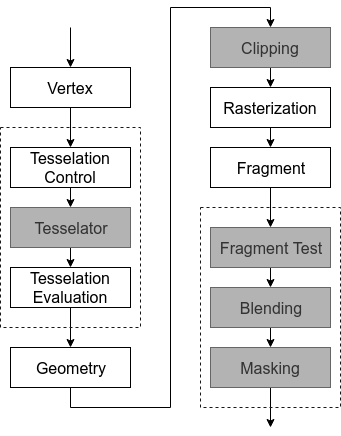
\includegraphics[width=0.3\textwidth]{opengl-pipeline.png}
  \end{center}
  \caption{The stages of the OpenGL rendering pipeline. White boxes represent stages that can be customised with shader code.}
  \label{fig:openglpipeline}
\end{figure}

For consistency, we refer to a step within the hardware rendering pipeline as a ``stage'', an invocation of the hardware pipeline as a ``pass'', and all invocations of the hardware pipeline to produce an image as a ``frame''. \\

Each of the customisable stages only accepts a single shader for each pass, making it difficult to separate, encapsulate, and ultimately combine behaviour. Furthermore, the steps required in order to change the shaders and shader inputs can be non-trivial and expensive to execute. \\

\begin{figure}[h]
  \begin{center}
    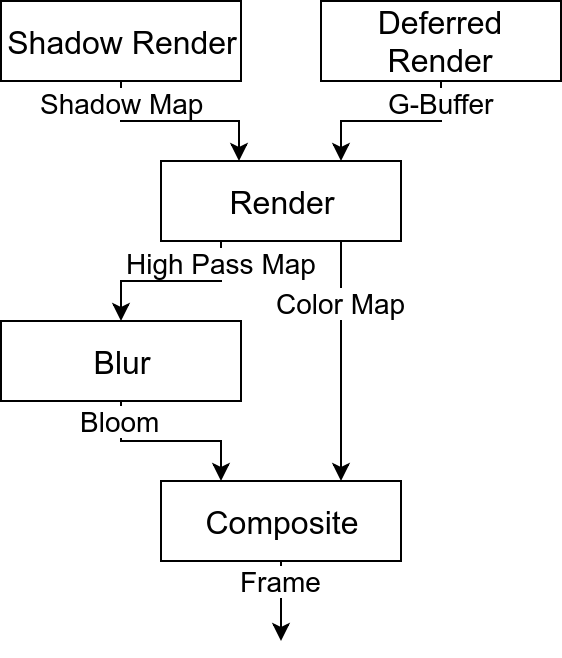
\includegraphics[width=0.3\textwidth]{render-pipeline.png}
  \end{center}
  \caption{A sample frame pipeline with shadow mapping, deferred rendering, and bloom. Each box represents a pass and each edge a texture buffer.}
  \label{fig:renderpipeline}
\end{figure}

The complexity of managing the graphics state and the order of rendering can be massively complicated for modern requirements. Rendering a frame often requires a multitude of passes, each with their own parameters and shared data. The rendering of each object within a pass can also differ, leading to even more state that needs to be correctly managed. \\

This results in a difficult challenge for modularity. We attempt to solve this challenge through several systems:

\begin{itemize}
\item A protocol for communicating information between a pass and the objects rendered within.
\item A protocol to connect the inputs, outputs, and parameters of different passes.
\item An algorithm to automatically allocate shared textures used as buffers between passes.
\end{itemize}

\section{Related Work}\label{relatedwork}
Courreges\cite{gtav} presents an in-depth analysis of the rendering procedure employed by the modern, high-production game GTA V. It illustrates the many passes to produce a final image, as well as their data dependencies. \\

Harada et al.'s work on Forward+\cite{forward+}\cite{forward+talk} also clearly illustrates the need for systems that support multi-pass rendering pipelines with complex data interaction schemes. \\

Gyrling\cite{fibers} presents an overview of the techniques used to perform parallel rendering in Naughty Dog's commercial engine. Individual stages within a pass, render passes of a frame, and multiple frame renderings are divided up into many small jobs that can run in parallel and are synchronised using counters on a shared structure. \\

The case study of the Unity game engine by Messaoudi et al\cite{unity} shows the availability of a set of fixed rendering pipelines that can be customised in a very limited extent with custom shaders. However, these shaders must fit into Unity's existing lighting and overall rendering model. While Unity does allow building a custom pipeline via their Scriptable Rendering Pipeline\cite{unitycustom}, they do not seem to offer any specific encapsulation or modularity features. \\

The work by He et al.\cite{components} introduces a framework for general encapsulation of shaders and their parameters into structures that minimise the overhead of changing GPU state while retaining the ability to dynamically compose shader parts. They do however not create a distinction between properties for the rendering of an object, and those for the rendering of an overall pass. \\

Foley et al.'s work on Spark\cite{spark} presents a high-level graph-based system for defining reusable and composable shader components. Their system shows a much more distanced view of the underlying graphics hardware than we attempt. Similar to He's work, they do not present a separation between object logic and pass logic. \\

In our previous work\cite{glsloop} we introduce a system to tie shader code to classes and compose behaviour through inheritance. We make use of this system and extend it to allow further control over rendering behaviour in individual passes.

\section{Overview}\label{overview}


\section{Passes}\label{passes}

\section{Pipelines}\label{pipelines}

\section{Allocation}\label{allocation}
In order to prepare the shader pipeline, several resources need to be allocated. Each shader stage needs a ``framebuffer,'' an OpenGL resource that allows one to render to off-screen textures. These framebuffers then need to have the required textures to render onto allocated as well. As each input and output from a pass can specify constraints on the texture's features, these constraints must be matched up for any connecting edges as well. Finally, in order to minimise memory usage we would like to re-use textures where possible.

Thus the allocation proceeds in three phases: reconciling texture constraints on edges between passes, computing how textures are shared between passes, and finally constructing all the necessary resources with the previously gathered information.

\subsection{Constraint Merging}\label{texture-constraints}
OpenGL textures include a massive amount of information.\cite{texparameter}\cite{teximage2d} When two ports are connected that specify different constraints on the texture properties, a join must be performed. Fortunately, a wide range of the texture property values are fundamentally incompatible, meaning that a lot of the logic can simply error. For simplicity and brevity, we will focus on the join operator for a single texture property here, the internal format. The internal format specifies how many colour channels the texture has, how many bits of precision each channel has, which format each channel has, as well as whether the texture is compressed or has sRGB gamma normalisation applied. \\

The list of specified texture formats is quite large.\cite{texinternalformat} Unfortunately OpenGL does not give us an interface to handle these formats in a way that lets us pick the individual features easily. Instead, each format is represented by a constant number, with no relation to the features that format includes. This means that we need to first destructure each format into a list of its features:

\begin{itemize}
\item \code{R}, \code{G}, \code{B}, \code{A} How many bits to use for each channel, and the format of the channel (normalised, float, integer, unsigned integer).
\item \code{depth} How many bits to use for the depth channel.
\item \code{stencil} How many bits to use for the stencil channel.
\item \code{shared} Whether bits are shared across the channel, and if so how many.
\item \code{features} Whether the format has compression, sRGB, RGTC, BPTC, SNORM, or UNORM features.
\end{itemize}

Once the texture format specifications are destructured, we can perform a join as follows.

\begin{step}
\item If the \code{features} and sharing are not the same, a join is impossible.
\item The \code{features} list of the output spec is set to the same as either of the specs.
\item If both include a \code{depth} component:
  \begin{step}
  \item The \code{depth} feature is set to the join of both.
  \item If either include a \code{stencil} feature, the \code{stencil} feature is set to the join of both.
  \end{step}
\item If both include a \code{stencil} component:
  \begin{step}
  \item The \code{stencil} feature is set to the join of both.
  \end{step}
\item If neither include a \code{depth} component:
  \begin{step}
  \item The \code{R} feature is set to the join of both.
  \item The \code{G} feature is set to the join of both.
  \item The \code{B} feature is set to the join of both.
  \item The \code{A} feature is set to the join of both.
  \end{step}
\item Otherwise a join is impossible.
\end{step}

Wherein the ``join of both'' is computed as the join of two channel formats as follows.

\begin{step}
\item If both include the format:
  \begin{step}
  \item If the channel format is not the same, a join is impossible.
  \item The channel bit depth is set to the maximum of both.
  \end{step}
\item If one includes the format, that format is returned.
\item Otherwise, the absence of the channel is indicated.
\end{step}

If the join is successful, we then re-encode the texture format specification into OpenGL's constant and use it in the real texture specification. Note that this join could texture format specifications that are not legal according to the OpenGL specification. However, this can only occur if one of the specs to join is already illegal. We thus deem it unnecessary to handle such cases.

\subsection{Port Allocation}\label{port-allocation}
In compilers, allocation of a graph of variables with use-relations is typically handled with a graph colouring algorithm. However, since we represent our graph in a different fashion than usual, with nodes having multiple distinct ports on which edges are connected, we devised a different kind of colouring algorithm to maximise texture sharing. \\

Given a set of nodes the allocation algorithm proceeds as follows.

\begin{step}
\item The set of unique texture specifications is computed by joining each port's texspec with every other and comparing for equality.
\item For each unique texture specification T:
  \begin{step}
  \item The nodes are sorted topologically.
  \item The number of colours is set to 0.
  \item For each node N:
    \begin{step}
    \item For each output port P of N:
      \begin{step}
      \item If P's texspec is joinable with T...
      \item The number of colours is increased
      \end{step}
    \end{step}
  \item An array is allocated to fit the number of colours. Each index of the array represents a colour and each value at the index whether the colour is currently available or unavailable.
  \item For each node N in \emph{reverse order}:
    \begin{step}
    \item For each input port P of N:
      \begin{step}
      \item For each neighbour port O of P:
        \begin{step}
        \item If O's texspec is joinable with T...
        \item and O does not yet have a colour...
        \item The first available colour is assigned to O.
        \item This colour is marked as unavailable.
        \end{step}
      \end{step}
    \item For each non-input port P of N:
      \begin{step}
      \item If P's texspec is joinable with T...
      \item and P does not yet have a colour...
      \item The first available colour is assigned to P.
      \item This colour is marked as unavailable.
      \end{step}
    \item For each port P of N:
      \begin{step}
      \item If P's texspec is joinable with T...
      \item and P has a colour...
      \item P's colour is marked as available.
      \end{step}
    \end{step}
  \end{step}
\end{step}

In other words, the algorithm proceeds backwards from the last node in the graph, marking predecessors' output ports with unique colours, then marking unconnected ports with unique colours, and finally marking all colours at its own output ports as available again. We repeat this process for each unique texture specification, each time ensuring we only consider ports that share that texture specification. \\

This algorithm is by no means efficient, but since pipeline allocation only has to happen during loading phases, we currently do not consider this to be a big problem. \\

Unfortunately print documents cannot yet display animations, so illustrating the algorithm in motion is not possible directly in the document. However, a brief animation of the pipeline illustrated in \autoref{fig:renderpipeline} is available online: \\

\href{https://raw.githubusercontent.com/Shinmera/talks/master/els2019-shader-pipeline/pipeline-allocation.gif}{https://raw.githubusercontent.com/Shinmera/talks/master/\\els2019-shader-pipeline/pipeline-allocation.gif}

\section{Conclusion}\label{conclusion}

\section{Further Work}\label{further-work}

\section{Acknowledgements}\label{acknowledgements}

\section{Implementation}\label{implementation}
An implementation of the proposed system can be found at
\\\href{https://github.com/Shirakumo/trial/blob/f34a79f0a6df21d1ed9259e85fbb3c7eed39352b/shader-pass.lisp}{https://github.com/Shirakumo/trial/blob/\\f34a79f0a6df21d1ed9259e85fbb3c7eed39352b/shader-pass.lisp}
\\\href{https://github.com/Shirakumo/trial/blob/f34a79f0a6df21d1ed9259e85fbb3c7eed39352b/pipeline.lisp}{https://github.com/Shirakumo/trial/blob/\\f34a79f0a6df21d1ed9259e85fbb3c7eed39352b/pipeline.lisp}
\\\url{https://github.com/Shinmera/flow} \\

A more in-depth discussion of the system can be found at
\\\url{https://reader.tymoon.eu/article/363}
\\\url{https://reader.tymoon.eu/article/364}

\bibliography{paper}
\end{document}

%%% Local Variables:
%%% mode: latex
%%% TeX-command-extra-options: "-shell-escape"
%%% TeX-master: t
%%% TeX-engine: luatex
%%% End:
